% Chapter Template

\chapter{Ensayos y resultados} % Main chapter title

\label{Chapter4} % Change X to a consecutive number; for referencing this chapter elsewhere, use \ref{ChapterX}
En este capítulo se describe el conjunto de ensayos realizadas sobre el sistema y se recopilan sus resultados.
Con este propósito, se explican las características del \textit{hardware} y el banco de pruebas que se emplearon.
Además, se explica cuáles son los criterios de evaluación para determinar la calidad de las respuestas de los
modelos extensos de lenguaje.
Finalmente, se hace un análisis global de los resultados, destacando el grado de mejora que ofrece el sistema así como
sus errores más comunes.

%----------------------------------------------------------------------------------------
%	SECTION 1
%----------------------------------------------------------------------------------------

\section{Entorno y banco de pruebas}
Los ensayos fueron ejecutados en un equipo de altas prestaciones, orientado a tareas de cómputo intensivo y procesamiento de modelos de lenguaje de gran tamaño.
Sus especificaciones son las siguientes:
\begin{itemize}
\item Memoria RAM: 64 GB.
\item Tarjeta gráfica: NVIDIA GeForce RTX4080 SUPER, con 16 GB de memoria RAM dedicada.
\item Procesador: AMD Ryzen9 7950X3D 16-Core.
\item Sistema Operativo: Windows 11.
\end{itemize}

Aunque se emplearon diversos \textit{worldbuildings} en el proceso iterativo de refinamiento de las instrucciones,
el contexto narrativo de prueba se basó exclusivamente en textos pertenecientes al mundo de ficción ``Aanrah'',
desarrollado por el autor Necrowmancer en la plataforma de WorldAnvil \cite{aanrah2024}.
Esta ambientación fue seleccionada por ofrecer una combinación equilibrada de complejidad conceptual,
léxico específico y coherencia interna, sin alcanzar un volumen excesivo de contenido.
Dicha elección refleja el tipo de entradas que previsiblemente introducirán los usuarios del sistema,
al tiempo que plantea un desafío suficientemente realista para los modelos extensos de lenguaje.
El corpus de referencia se encuentra detallado en el Anexo(FALTA REFERENCIA).

%----------------------------------------------------------------------------------------
%	SECTION 2
%----------------------------------------------------------------------------------------

\section{Pruebas de procesamiento de ficheros}
Para comprobar el funcionamiento del procesamiento de los ficheros sin depender del módulo de procesamiento de peticiones \textit{web},
se implementaron varias celdas en un \textit{notebook} de Jupyter.
Esta solución no solo permite evaluar de forma controlada el comportamiento del módulo,
sino que además cumple con los criterios de pruebas automatizadas exigidos por el cliente.

Además, se formateó el contexto narrativo de prueba en los tres tipos de fichero aceptados: txt, docx y pdf.
El funcionamiento del módulo quedó validado tras comprobar que el texto extraído de todos los ficheros es idéntico,
tal y como se muestran en las figuras \ref{fig:txt-read-test}, \ref{fig:docx-read-test} y \ref{fig:pdf-read-test}.
Se aprecian diferencias de formato en el archivo pdf, pero su contenido coincide.

\begin{figure}[htbp]
	\centering
	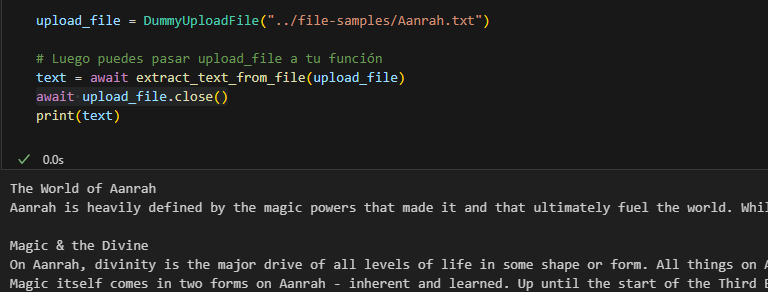
\includegraphics[width=0.9\textwidth]{./Figures/file-read-test-txt.png}
	\caption{Prueba de lectura de ficheros txt.}
	\label{fig:txt-read-test}
\end{figure}

\begin{figure}[htbp]
	\centering
	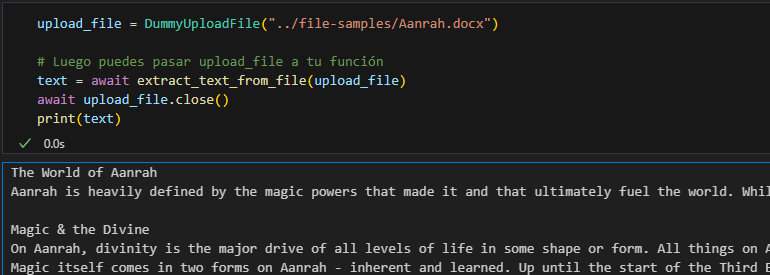
\includegraphics[width=0.9\textwidth]{./Figures/file-read-test-docx.png}
	\caption{Prueba de lectura de ficheros docx.}
	\label{fig:docx-read-test}
\end{figure}

\begin{figure}[htbp]
	\centering
	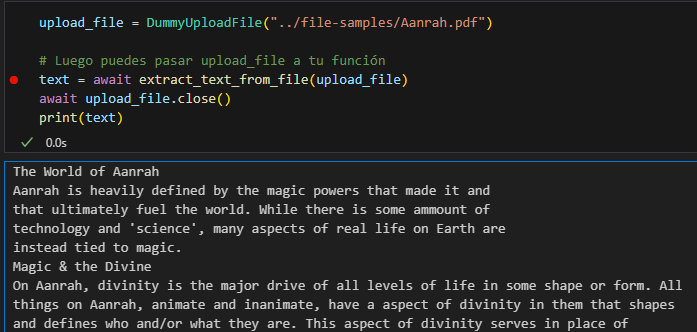
\includegraphics[width=0.9\textwidth]{./Figures/file-read-test-pdf.png}
	\caption{Prueba de lectura de ficheros pdf.}
	\label{fig:pdf-read-test}
\end{figure}

%----------------------------------------------------------------------------------------
%	SECTION 3
%----------------------------------------------------------------------------------------
\pagebreak
\section{Pruebas de procesamiento de peticiones web}
Durante la fase de implementación se llevaron a cabo pruebas incrementales que incluyeron
la verificación de la correcta carga del HTML, la recepción de las peticiones junto con los archivos adjuntos,
la lectura del contenido y, finalmente,
la integración completa del flujo de comunicación entre el usuario y el modelo extenso de lenguaje.
Cuando una petición se procesa correctamente, la información se envía de vuelta a la interfaz \textit{web},
donde se muestra en un cuadro de texto.

En la figura~\ref{fig:web-test} se muestra el resultado de una petición en la que,
con fines de prueba, se omitió el envío al módulo LLM
y en su lugar se devolvió directamente al usuario el contenido del fichero adjunto.

\begin{figure}[htbp]
	\centering
	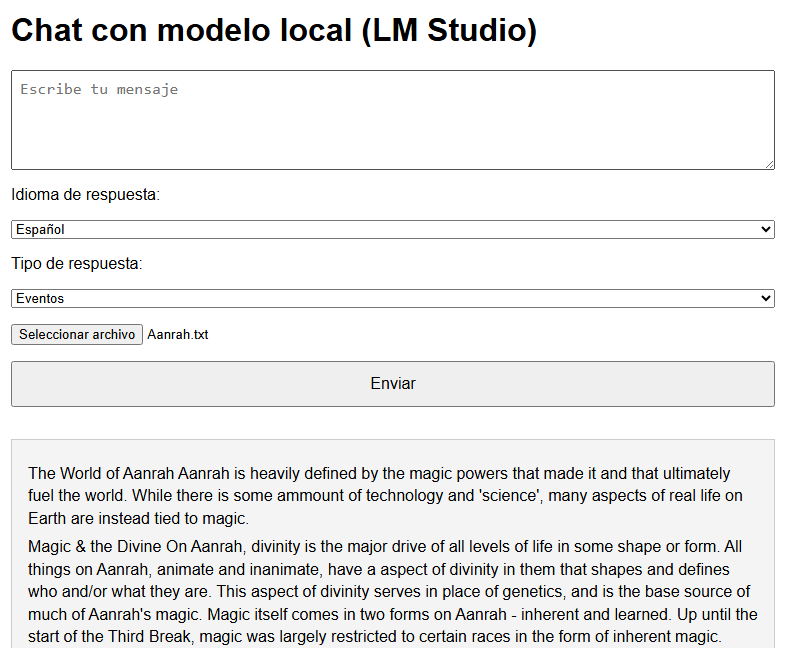
\includegraphics[width=1\textwidth]{./Figures/web-test.png}
	\caption{Prueba de envío de peticiones REST.}
	\label{fig:web-test}
\end{figure}

En las pruebas de los siguientes apartados se muestran múltiples figuras de la interfaz con el flujo completo de datos.

%----------------------------------------------------------------------------------------
%	SECTION 4
%----------------------------------------------------------------------------------------
\section{Método para valorar la salida de los modelos extensos de lenguaje}
En este apartado se explica la lógica que se siguió para valorar la calidad de las respuestas
generadas por el modelo de lenguaje.
Este proceso presenta una dificultad inherente:
debido a la naturaleza de los casos de uso del sistema, esta puntuación es completamente subjetiva.
Conceptos como “adecuación”, “originalidad” o “interés narrativo” no pueden medirse de forma objetiva ni automática,
lo que limita la posibilidad de una evaluación completamente reproducible.
Por ello, la validación fue realizada de forma manual, basándose en mi propio criterio como desarrollador del sistema.

Una vez aclarado este aspecto, las pruebas se estructuraron de forma que pudieran reproducirse de manera sencilla y sistemática.
En todas las evaluaciones se emplea el mismo fichero adjunto, que contiene el contexto narrativo base,
y se combina con cada tipo de elemento de \textit{worldbuilding} que se desea generar.
Este enfoque se aplica de forma consistente a todos los modelos extensos de lenguaje.
Adicionalmente, sobre este mismo conjunto de pruebas se compararán dos escenarios:
uno en el que se utiliza la ingeniería de \textit{prompting} desarrollada en este trabajo,
y otro en el que dicha técnica no se aplica.
Este constraste permitirá evaluar el impacto real de las instrucciones
refinadas sobre los modelos.

Para valorar la salida del modelo se emplearon los siguientes criterios:
\begin{itemize}
\item \textbf{Adecuación contextual}: se verifica que los elementos generados respeten el tono, estilo y detalles del contexto narrativo original.
\item \textbf{Pertinencia temática}: los resultados deben estar alineados con la categoría seleccionada
(por ejemplo, si se ha elegido ``personajes'', la salida no debe incluir ubicaciones o eventos).
\item \textbf{Originalidad}: se valora la capacidad del modelo para proponer ideas nuevas sin repetir explícitamente el contenido del fichero.
\item \textbf{Diversidad}: se analiza si la lista contiene variedad en las propuestas y evita repeticiones o elementos demasiado similares.
\item \textbf{Idioma}: se indica si el modelo acepta texto en español. 
\item \textbf{Consistencia}: analiza la inestabilidad en la respuesta de los modelos,
teniendo en cuenta que todos fueron configurados con una temperatura de 0,7 sobre 1. 
\item \textbf{Errores}: se listan los errores encontrados en las pruebas y se analiza el impacto que tienen.
\end{itemize}

%----------------------------------------------------------------------------------------
%	SECTION 5
%----------------------------------------------------------------------------------------
\section{Pruebas con modelos generalistas y \textit{prompting} poco preciso}
Esta sección analiza el rendimiento de los modelos que no han sido ajustados específicamente
para tareas de ambientación narrativa y que carecen de un refinamiento adecuado en las instrucciones.
El objetivo es simular los resultados que podrían obtenerse si una persona sin experiencia en ingeniería de
\textit{prompting} utilizara las opciones más comunes disponibles en línea.

Para lograr esto, se desactivó el módulo de \textit{prompts} y se bloquearon algunos controles de la interfaz
\textit{web} para que solo aceptara el fichero adjunto, el cuadro de texto y el selector de idiomas.
En la figura \ref{fig:prompt-test} se muestra
como el modelo responde libremente a la entrada del usuario.
Una vez validada la funcionalidad, todas las instrucciones se simplificaron en una única frase:
``dame una lista de diez nuevos'' seguido del elemento narrativo que se quería obtener.
\pagebreak
\begin{figure}[htbp]
	\centering
	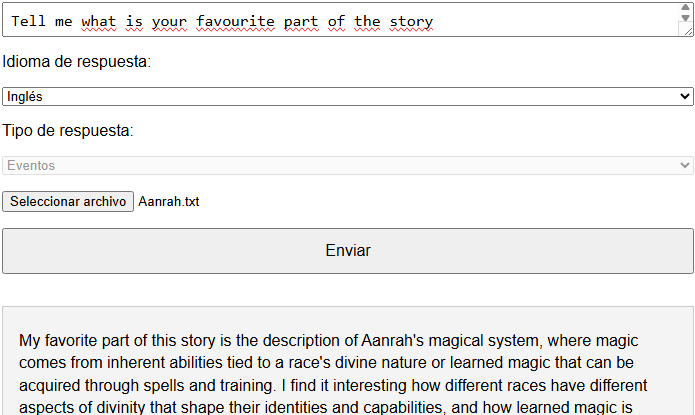
\includegraphics[width=1\textwidth]{./Figures/promp-testing.png}
	\caption{Prueba de desconexión del módulo generador de instrucciones.}
	\label{fig:prompt-test}
\end{figure}

\subsection{Resultados de \textit{deepseek}}
En el caso de \textit{deepseek}, presentó una adaptación al contexto narrativo aceptable y se ciñó correctamente al
tipo de elemento narrativo que se especificó.
No obstante, su desempeño en relación a la variedad de las ideas fue baja al presentar puntos muy similares entre sí.
Este problema fue especialmente notable en el caso de los personajes y eventos.
Por último, la consistencia de sus respuestas varió en ocasiones.
Esto significa que su sensibilidad a la temperatura es bastante alta.
El modelo puede responder en español pero los errores de traduccion y alucinaciones son frecuentes,
tal y como se muestra en la figura \ref{fig:deepseek-esp}:

\begin{figure}[htbp]
	\centering
	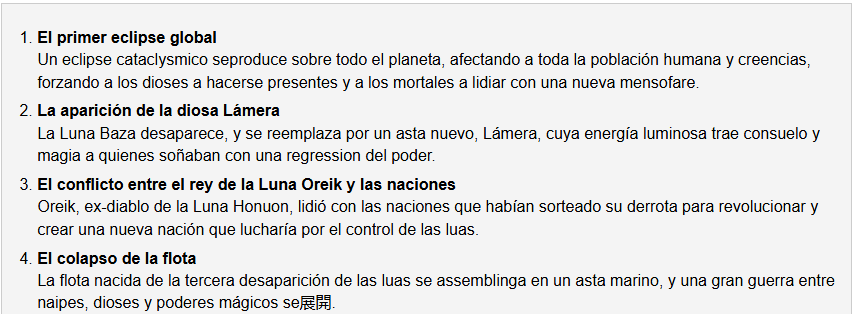
\includegraphics[width=1\textwidth]{./Figures/deepseek-noprompt-spanish.png}
	\caption{Resultado en español de \textit{deepseek} para eventos.}
	\label{fig:deepseek-esp}
\end{figure}
\pagebreak
\subsection{Resultados de \textit{mistral}}
El modelo generalista de \textit{mistral} no consiguió la misma calidad en sus respuestas.
Las propuestas, aunque tienen relación con el contexto de la historia,
es una conexión sin demasiada profundidad en los detalles ni en su variedad.
En los casos de geografía y asentamientos, su relacion con el contexto es mínima o nula
(ver figura \ref{fig:mistral-geo}), lo que sugiere que su entrenamiento no le permite ser
flexible en la generación de contenido narrativo sin instrucciones previas.
Este modelo pierde completamente el contexto al responder en español,
lo que provoca que utilice referencias reales,
como ciudades de Estados Unidos, personajes históricos o festividades internacionales.

\begin{figure}[htbp]
	\centering
	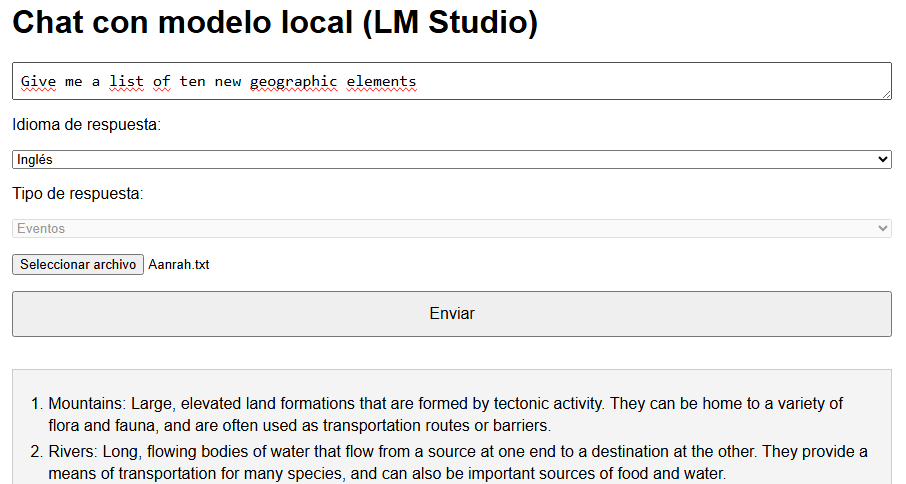
\includegraphics[width=1\textwidth]{./Figures/mistral-noprompt-geography.png}
	\caption{Resultado de \textit{mistral} para geografía}
	\label{fig:mistral-geo}
\end{figure}

%----------------------------------------------------------------------------------------
%	SECTION 6
%----------------------------------------------------------------------------------------
\section{Pruebas con modelos reentrenados y \textit{prompting} poco preciso}
Análogamente a la sección anterior, se llevaron a cabo pruebas equivalentes
sobre los modelos refinados con el fin de evaluar su rendimiento.
Los resultados permiten establecer una comparación entre estos LLM
y los modelos generalistas.

\subsection{Resultados de \textit{writing-roleplay}}
El modelo de \textit{writing-roleplay} funcionó correctamente en la generación de eventos,
comprendiendo adecuadamente el contexto y ofreciendo ideas interesantes.
Sin embargo, presentó problemas en el resto de elementos narrativos.
A pesar de que aporta una variedad aceptable y una ambientación de fantasía correcta,
su respuesta se ajusta más a un contenido predefinido que a algo adaptado a la ambientación
narrativa del fichero adjunto.
Finalmente, fue notoria la inconsistencia del modelo a la temperatura a la que fue configurado,
ya que ocasionalmente repetía información en vez de aportar ideas nuevas.

\subsection{Resultados de \textit{worldbuilder}}
En el caso de \textit{worldbuilder},
su comprensión de la entrada destacó sobre las alternativas generalistas,
aportando ideas con una relación profunda con el contexto de entrada
(Figura \ref{fig:worldbuilder-settle}).
Sin embargo, el modelo también tiene una sensibilidad alta de temperatura
y ocasionalmente puede ignorar la ambientación al generar nuevo contenido.
Algo único de este LLM es que puede llegar a dar consejos al usuario de cómo
hacer la construccion de mundos, con diversas técnicas y explicaciones,
en vez de dar una lista de nuevas ideas.
También es el único que no puede dar respuestas en español.

\begin{figure}[htbp]
	\centering
	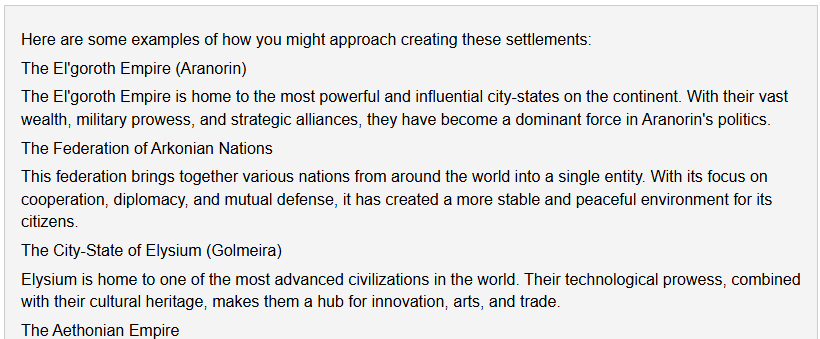
\includegraphics[width=1\textwidth]{./Figures/worldbuilder-noprompt-settlements.png}
	\caption{Resultado de \textit{worldbuilder} para asentamientos}
	\label{fig:worldbuilder-settle}
\end{figure}

\subsection{Resultados de \textit{arliai-rpmax}}
Finalmente, el modelo \textit{arliai-rpmax} fue el que mejor desempeño demostró. 
Se ajustó al contexto de entrada y profundizó en las respuestas de forma aceptable.
Donde también destacó es en la capacidad de generar texto en español sin verse afectado
en la calidad del mensaje. 

A nivel global, todos los LLM funcionaron bien para los eventos y las localizaciones
mientras que carecieron de originalidad en la generación de personajes y geografía.
En la figura \ref{fig:rpmax-chars} se muestra un ejemplo de este fenómeno.

\begin{figure}[htbp]
	\centering
	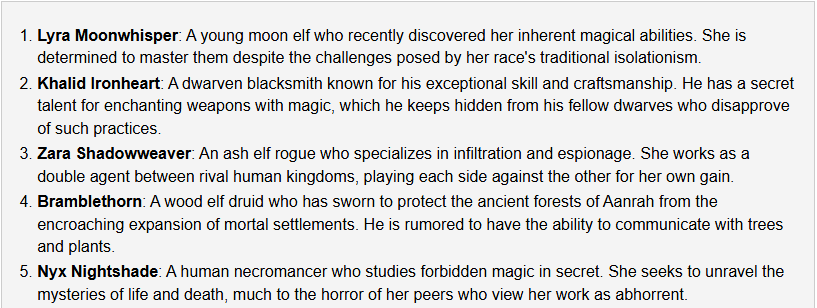
\includegraphics[width=1\textwidth]{./Figures/rpmax-noprompt-chars.png}
	\caption{Resultado de \textit{arliai-rpmax} para personajes}
	\label{fig:rpmax-chars}
\end{figure}

%----------------------------------------------------------------------------------------
%	SECTION 7
%----------------------------------------------------------------------------------------
\section{Pruebas con modelos generalistas y \textit{prompting} preciso}
Esta sección analiza el rendimiento de modelos generalistas que no han sido específicamente
ajustados para tareas de ambientación narrativa.
A diferencia de enfoques anteriores sin refinamiento,
en este caso se emplea \textit{prompting} preciso para maximizar la capacidad del modelo.
El objetivo es evaluar qué tan eficaz puede ser una estrategia de instrucciones
al trabajar con modelos accesibles públicamente.

Para ello, se hace uso del módulo de instrucciones y la página \textit{web}
en su versión final. Tal y como se demuestra en la figura \ref{fig:full-prompt-test},
el sistema construye la instrucción de forma transparente para el usuario, por lo que
solo es necesario que se adjunte el fichero con el contexto narrativo.

\begin{figure}[htbp]
	\centering
	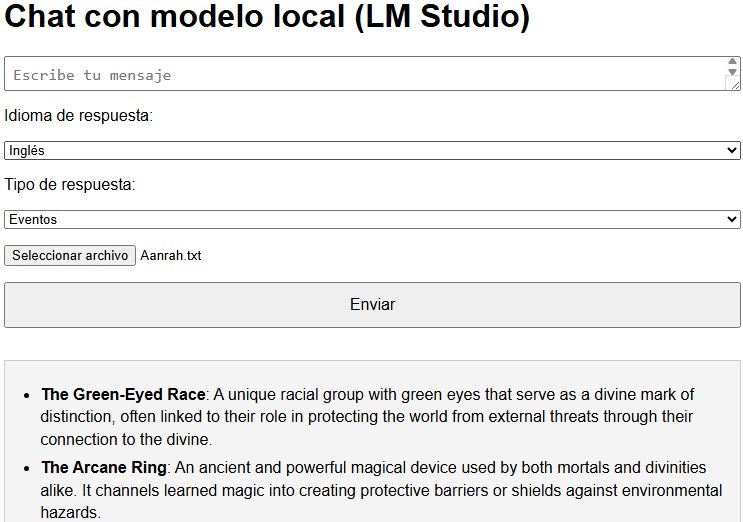
\includegraphics[width=0.85\textwidth]{./Figures/full-promp-testing.png}
	\caption{Prueba de la versión definitiva del sistema.}
	\label{fig:full-prompt-test}
\end{figure}

\subsection{Resultados de \textit{deepseek}}
Este modelo tuvo una mejora notable en la calidad de sus respuestas, tanto a nivel de profundidad
contextual como en variedad de las ideas que aporta.
El modelo es capaz de relacionar muchos más elementos de la ambientación narrativa y
plasmarlo en las propuestas tanto en los eventos como en los personajes y geografía
(ver figura \ref{fig:deepseek-prompt-char}).
La consistencia de las respuestas no varió,
produciéndose raramente errores de formato y temática.
El coste de responder en español también se vió reducido.

\begin{figure}[htbp]
	\centering
	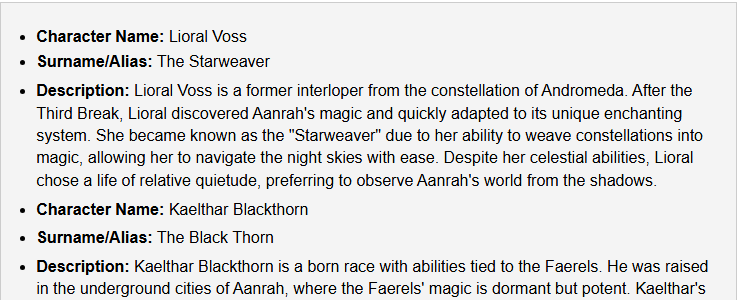
\includegraphics[width=1\textwidth]{./Figures/deepseek-prompt-characters.png}
	\caption{Resultado de \textit{deepseek} para personajes.}
	\label{fig:deepseek-prompt-char}
\end{figure}
\pagebreak
\subsection{Resultados de \textit{mistral}}
\textit{Mistral} no se adaptó adecuadamente a la ingeniería de instrucciones y 
se volvió muy inconsistente.
Cuando interpreta correctamente las instrucciones,
muestra una ligera mejora en comparación a instrucciones básicas.
Entre los errores más comunes se encuentra la duplicación de la lista y
la perdida sustancial de la temática en la respuesta,
lo que provoca que exceda los 10 elementos especificados por defecto
y además guarden muy poca relación con el contexto general.
Por último, el modelo pierde completamente su capacidad de responder en español.

\begin{figure}[htbp]
	\centering
	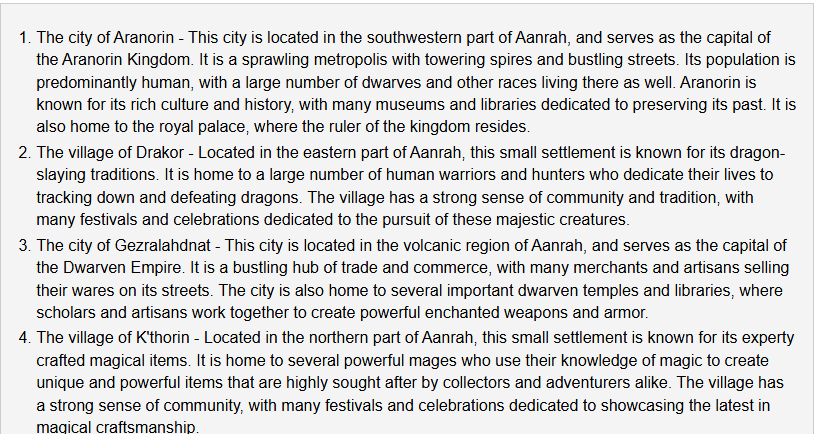
\includegraphics[width=1\textwidth]{./Figures/mistral-prompt-locations.png}
	\caption{Resultado de \textit{mistral} para localizaciones.}
	\label{fig:mistral-prompt-locations}
\end{figure}

%----------------------------------------------------------------------------------------
%	SECTION 8
%----------------------------------------------------------------------------------------
\section{Pruebas con modelos reentrenados y \textit{prompting} preciso}
Finalmente, se realizan las pruebas sobre los modelos refinados e instrucciones precisas
y se analizan sus resultados.
\subsection{Resultados de \textit{writing-roleplay}}
La compresión del LLM mejoró ligeramente,
aunque esta mejora fue evidente principalmente en la generación de eventos.
En cambio, en el resto de categorías el rendimiento se mantuvo similar al anterior.
En varias ocasiones el modelo interpreta que debe generar una lista de varias decenas de puntos
y esto provocó bloqueos en el modelo.

\begin{figure}[htbp]
	\centering
	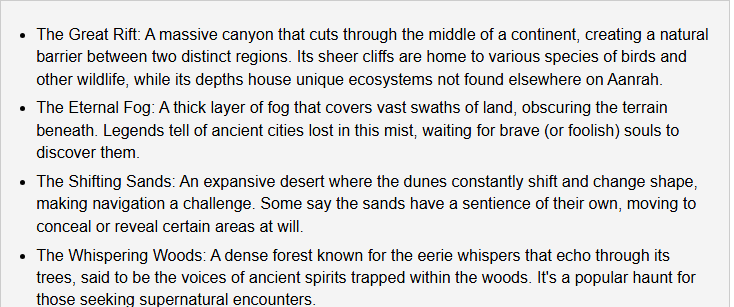
\includegraphics[width=1\textwidth]{./Figures/writing-prompt-geography.png}
	\caption{Alucinación de \textit{writing-roleplay} para geografía.}
	\label{fig:writing-geography}
\end{figure}

\subsection{Resultados de \textit{worldbuilder}}
Con las nuevas instrucciones el modelo muestra
una leve mejora en la comprensión del contexto de entrada
y queda plasmada en la generación.
No obstante, en el apartado de geografía y localizaciones no mostró ninguna mejora.
En esta configuración también sufrió alucinaciones, como se muestra en la figura \ref{fig:worldbuilder-hallucination},
que complejizaron el listado y devolvió varias listas con diferentes categorías.

\begin{figure}[htbp]
	\centering
	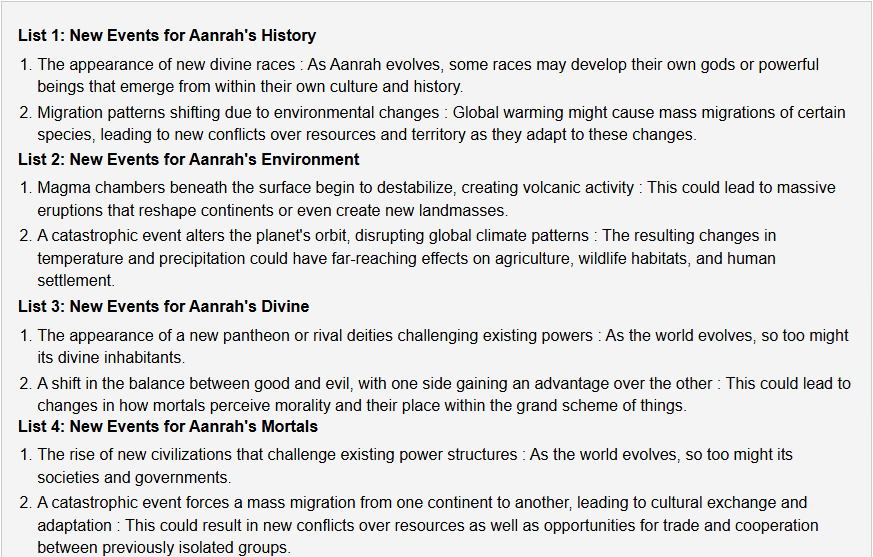
\includegraphics[width=1\textwidth]{./Figures/worldbuilder-hallucination-events.png}
	\caption{Alucinación de \textit{worldbuilder} en la generación de eventos.}
	\label{fig:worldbuilder-hallucination}
\end{figure}

\subsection{Resultados de \textit{arliai-rpmax}}
Gracias al refinamiento de los prompts,
mejoró significativamente su comprensión e inclusión del contexto,
y resultó en respuestas excepcionales.
También destacó por su capacidad de generar texto en español
manteniendo una calidad constante en el mensaje.

\begin{figure}[htbp]
	\centering
	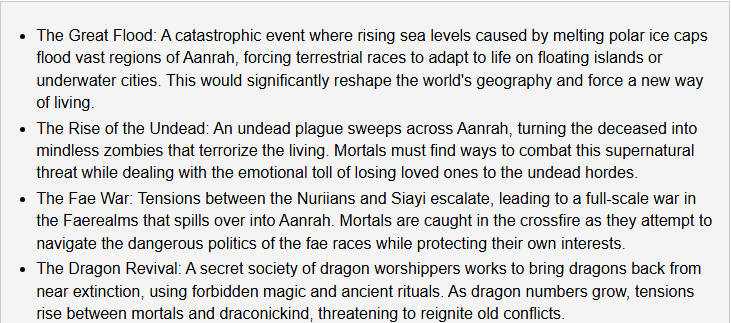
\includegraphics[width=1\textwidth]{./Figures/rpmax-prompt-events.png}
	\caption{Resultado de \textit{arliai-rpmax} en la generación de eventos.}
	\label{fig:rpmax-events}
\end{figure}

A nivel global, se observó una mejora clara en la generación de eventos de todos los LLM,
en comparación con evaluaciones anteriores.
Sin embargo, los resultados no fueron tan positivos en lo referente a la creación de personajes,
la geografía y las localizaciones,
donde los modelos continuaron mostrando una falta de originalidad y variedad.
Queda por estudiar si este fenómeno es producto del sobreentrenamiento o escasez de información
en la ambientación narrativa mpleada en los ensayos.

%----------------------------------------------------------------------------------------
%	SECTION 9
%----------------------------------------------------------------------------------------
\section{Interpretación de resultados}